\newpage
\section{Designing for Manufacturability and Feasibility Audits}
\label{app:details}
This appendix preserves the hardware audits and validation examples from the
original campaign. Its RTL tapes, Timeloop mappings, and physical proxy gates
retain that campaign's workload and hardware scope. The native full-inference
extension has separate execution and service contracts in
Appendix~\ref{app:native_provenance}; these earlier audits do not establish its
memory-interface timing or physical implementation.


\subsection{Five Levels of Validation}
\label{app:validation}
The original campaign uses five levels of modeled feasibility validation.

\begin{enumerate}
    \item Roofline Auditor: A deterministic Roofline Auditor checks physical feasibility by comparing
each LP-predicted latency against the lower bound
\begin{equation}
    \mathrm{LB} = \max\!\left(t_{\mathrm{floor}},\;
    t_{\mathrm{memory}}\right),
\end{equation}
where $t_{\mathrm{floor}}$ is the mapper-derived compute floor of
\cref{eq:floor_construction} and $t_{\mathrm{memory}}$ is post-placement
off-chip traffic divided by available memory bandwidth.
The audit additionally reports the compute-floor tightness
$\rho_{\mathrm{comp}}$ and memory utilization; values above 1 would indicate a
physically impossible prediction. Neither ratio is a model FLOPs utilization,
which \cref{app:mfu} distinguishes.
The original campaign's audited results have zero roofline lower-bound violations;
\cref{app:mfu} gives the detailed checks.

\item Campaign Validator: A deterministic Campaign Validator legalizes LLM-proposed architectural
neighbourhoods by enforcing hardware ranges, power-of-two constraints,
TDP and area caps, MAC caps, CGM feasibility floors, and
compute/bandwidth coupling constraints before Vizier is permitted to
sample candidates.
\item Causal Ledger:
The Causal Ledger records each LLM hypothesis, intervention, and observed
outcome, making the search loop fully auditable and preventing repeated
exploration of empirically invalid regions.
\item Solver diagnostics:
The LP solver reports mathematical solver diagnostics such as primal and dual
residuals, duality gap, rounding gap, and fractionality. 
In our experiments LP solutions are not treated as trustworthy unless both the relaxation and the rounded design are numerically well behaved.
\item Pre-RTL Feasibility Gates: Original-campaign designs pass six first-order
screens for pin count, power density, logic depth, and related resource costs.
\cref{app:gates} provides their definitions. Passing these proxies does not
constitute physical-design sign-off.
\end{enumerate}


\subsection{Compute-Floor and Roofline Tightness Audits}
\label{app:mfu}
\paragraph{What this audit reports, and what it is not.}
The original campaign's audit column records a \emph{tightness} ratio, not a
model-FLOP utilization. Write $T_{\mathrm{LP}}$ for the LP-predicted latency of
a cell: its modeled execution time, never the optimizer's runtime. The archived
quantity is
\begin{equation}
    \rho_{\mathrm{comp}}
    = \frac{t_{\mathrm{floor}}}{T_{\mathrm{LP}}},
    \label{eq:mfu_audit}
\end{equation}
which we call \emph{compute-floor tightness}. Earlier versions of this appendix
labelled $\rho_{\mathrm{comp}}$ ``MFU''. We retire that label and leave every
archived number unchanged: the audited values in \cref{app:blueprints} and
\cref{app:deficit} are $\rho_{\mathrm{comp}}$.

The label has to go because of the numerator. The auditor does not count useful
model arithmetic from the graph. It derives a FLOP total from the per-operator
Timeloop tile minima, $F = 2\,M_{\mathrm{ref}}\sum_c T_{\min}(c)$, and divides
by the candidate chip's arithmetic rate, so that
\begin{equation}
    t_{\mathrm{floor}}
    = \sum_c T_{\min}(c)\cdot\frac{M_{\mathrm{ref}}}{M},
    \label{eq:floor_construction}
\end{equation}
with $M$ the candidate's MAC count and $M_{\mathrm{ref}}$ the reference
geometry's. Now $\sum_c T_{\min}(c)$ is a \emph{mapping} result: it already
carries the reference datapath's tile padding and mapping inefficiency. So
$t_{\mathrm{floor}}$ is not $F_{\mathrm{model}}/C_{\mathrm{peak}}$, and
$\rho_{\mathrm{comp}}$ is not the model FLOPs utilization of
\cref{sec:reported_quantities}. The two ratios would coincide only if the
numerator were the useful-arithmetic count at the same peak rate and phase
boundary, and here it is not. Accordingly $\rho_{\mathrm{comp}} = 1$ says the LP
objective has reached the mapper's per-operator floor at the selected geometry.
That is a statement about scheduling slack, not about how much of the silicon's
arithmetic the model keeps busy.

\paragraph{Roofline-bound tightness.}
The auditor separately checks the lower bound
\begin{equation}
    T_{\mathrm{LP}}
    \;\geq\;
    \mathrm{LB} = \max\!\left(t_{\mathrm{floor}},\; t_{\mathrm{memory}}\right),
    \label{eq:roofline_lb}
\end{equation}
where $t_{\mathrm{memory}}$ is total scheduled bytes divided by peak bandwidth,
and enforces $\texttt{roof\_ratio} = \mathrm{LB}/T_{\mathrm{LP}} \le 1.001$ as
the pass criterion. Only the ratio built on this maximum,
$\rho_{\mathrm{roof}} = \mathrm{LB}/T_{\mathrm{LP}}$, deserves the name
\emph{roofline} tightness. The distinction matters in precisely the regime the
compute-only ratio hides: a memory-bound cell can sit on its roofline bound,
$\rho_{\mathrm{roof}} \to 1$, while its compute-floor ratio stays small.
Calling $\rho_{\mathrm{comp}}$ a roofline-tightness ratio, as earlier versions
of this appendix did, is imprecise whenever memory is the active limitation.

\paragraph{What the audit establishes.}
A value $\rho_{\mathrm{comp}} > 1$, or an LP latency below
$\max(t_{\mathrm{floor}}, t_{\mathrm{memory}})$, would indicate a physically
impossible prediction or a cost-model violation; the original campaign's
audited cells show no such violation. That is a necessary consistency
condition, and it is all this audit supplies. It does not establish
realizability, silicon timing accuracy, or optimality, and a real
implementation would generally fall below either bound through pipeline
bubbles, NoC contention, SRAM bank conflicts, control overhead, imperfect
scheduling and compiler effects.

\paragraph{Predicted versus measured utilization.}
Model FLOPs utilization is defined in \cref{sec:reported_quantities} as
$F_{\mathrm{model}}/(C_{\mathrm{peak}}T)$. Predicted and measured variants are
the same metric under different timing evidence,
\begin{equation}
    \mathrm{MFU}_{\mathrm{pred}}
    = \frac{F_{\mathrm{model}}}{C_{\mathrm{peak}}T_{\mathrm{pred}}},
    \qquad
    \mathrm{MFU}_{\mathrm{meas}}
    = \frac{F_{\mathrm{model}}}{C_{\mathrm{peak}}T_{\mathrm{meas}}},
    \label{eq:mfu_measured}
\end{equation}
and forming either needs only an analytical count of useful model arithmetic
and one execution time. Hardware counters explain where utilization is lost but
are not required to compute the ratio; an earlier version of this appendix
implied otherwise. A cycle-accurate simulator supplies a \emph{simulated} $T$,
which we would report as such and not as a silicon measurement. For the present
designs no executable implementation of the selected hardware/schedule pair
exists, so we report $\mathrm{MFU}_{\mathrm{pred}}$ against the recovered
execution's modeled latency and never a measured figure. Two conventions must
travel with any such number. The FLOP-counting rule, because padding,
rematerialized arithmetic and inactive experts are charged in time but are not
credited as useful work; and the precision of $C_{\mathrm{peak}}$, which must
match the arithmetic actually modeled, so an FP8-stored but BF16-computed path
takes the BF16 capability rather than an FP8 peak. Where one
multiply--accumulate counts as two FLOPs, numerator and denominator follow that
convention together.

\paragraph{Relation to FAST.}
FAST reports \emph{compute utilization}, defined there as a fraction of peak
throughput, and neither names nor specifies MFU; its modeled TPU-v3 entry is
$0.14$ on EfficientNet-B7~\citep{zhang_fast}. We therefore make no claim to
reproduce a FAST MFU definition. The tightness ratios $\rho_{\mathrm{comp}}$
and $\rho_{\mathrm{roof}}$ are not that quantity and are not comparable to it:
a utilization comparison would require one useful-work count and one peak
convention applied to both arms.

\begin{table}[ht!]
\centering
\caption{Single Workloads of Vizier-discovered hardware configuration.
$\rho_{\mathrm{comp}} = t_{\mathrm{floor}} / T_{\mathrm{LP}}$
is a compute-floor tightness ratio (see Eq.~\ref{eq:mfu_audit}), not a measured
hardware utilization and not the model FLOPs utilization of
\cref{sec:reported_quantities}. $\rho_{\mathrm{comp}} = 1.000$ means the LP hit the mapper-derived
compute floor. \emph{Compute-bound}: $\mathrm{obj} \approx t_{\mathrm{compute}}$.
\emph{Memory-bound}: $\mathrm{obj} \approx t_{\mathrm{memory}}$, $\rho_{\mathrm{comp}} < 1$.
\emph{Above-roofline}: obj exceeds both floors; expected for Static on hard cells,
unexpected for fixed-tile/joint-tile. Two cells (Llama-3 70B and DeepSeek-V3 under Static) had no
physically valid trial and are marked infeasible.}
\label{tab:exp1_roofline}
\resizebox{\textwidth}{!}{%
\begin{tabular}{llrrrrrrrrll}
\toprule
\textbf{Method} & \textbf{Model} &
\textbf{MACs} & \textbf{BW} &
\textbf{Speedup} & \textbf{Obj cycles} &
\textbf{Comp.\ floor} & \textbf{Mem.\ floor} &
$\boldsymbol{\rho_{\mathrm{comp}}}$ & \textbf{obj/lb} &
\textbf{Binding} & \textbf{Verdict} \\
\midrule
\multicolumn{12}{l}{\textit{Static FAST ILP}} \\
\midrule
Static & EN-B1       & 32{,}768  & 64   & 1.12  & $2.757\times10^{7}$ & $2.757\times10^{7}$ & $4.236\times10^{6}$ & 1.000 & 1.000 & compute-bound   & OK \\
Static & EN-B2       & 65{,}536  & 64   & 1.93  & $2.576\times10^{7}$ & $2.576\times10^{7}$ & $5.474\times10^{6}$ & 1.000 & 1.000 & compute-bound   & OK \\
Static & EN-B3       & 32{,}768  & 64   & 1.25  & $7.905\times10^{7}$ & $7.905\times10^{7}$ & $7.552\times10^{6}$ & 1.000 & 1.000 & compute-bound   & OK \\
Static & EN-B4       & 65{,}536  & 64   & 2.25  & $1.045\times10^{8}$ & $1.045\times10^{8}$ & $1.372\times10^{7}$ & 1.000 & 1.000 & compute-bound   & OK \\
Static & EN-B5       & 32{,}768  & 64   & 1.31  & $4.938\times10^{8}$ & $4.938\times10^{8}$ & $2.279\times10^{7}$ & 1.000 & 1.000 & compute-bound   & OK \\
Static & EN-B6       & 32{,}768  & 64   & 1.10  & $9.952\times10^{8}$ & $9.952\times10^{8}$ & $3.505\times10^{7}$ & 1.000 & 1.000 & compute-bound   & OK \\
Static & EN-B7       & 131{,}072 & 64   & 3.60  & $5.153\times10^{8}$ & $5.153\times10^{8}$ & $5.280\times10^{7}$ & 1.000 & 1.000 & compute-bound   & OK \\
Static & Llama-1 13B & 32{,}768  & 1024 & 1.07  & $2.705\times10^{10}$& $2.705\times10^{10}$& $2.981\times10^{7}$ & 1.000 & 1.000 & compute-bound   & OK \\
Static & Llama-1 65B & 65{,}536  & 128  & 0.61  & $2.377\times10^{11}$& $6.744\times10^{10}$& $9.514\times10^{8}$ & 0.284 & 3.525 & above-roofline  & loose (expected) \\
Static & Llama-3 70B & --         & --    & --     & --                   & --                   & --                   & --     & --     & --               & infeas \\
Static & DeepSeek-V3 & --         & --    & --     & --                   & --                   & --                   & --     & --     & --               & infeas \\
\midrule
\multicolumn{12}{l}{\textit{Dynamic fixed-tile LP (time-indexed + rematerialisation)}} \\
\midrule
fixed-tile & EN-B1       & 65{,}536  & 64  &  2.24 & $1.379\times10^{7}$ & $1.379\times10^{7}$ & $4.236\times10^{6}$ & 1.000 & 1.000 & compute-bound & OK \\
fixed-tile & EN-B2       & 131{,}072 & 64  &  3.87 & $1.288\times10^{7}$ & $1.288\times10^{7}$ & $5.474\times10^{6}$ & 1.000 & 1.000 & compute-bound & OK \\
fixed-tile & EN-B3       & 131{,}072 & 64  &  4.99 & $1.976\times10^{7}$ & $1.976\times10^{7}$ & $7.552\times10^{6}$ & 1.000 & 1.000 & compute-bound & OK \\
fixed-tile & EN-B4       & 131{,}072 & 64  &  4.51 & $5.225\times10^{7}$ & $5.225\times10^{7}$ & $1.372\times10^{7}$ & 1.000 & 1.000 & compute-bound & OK \\
fixed-tile & EN-B5       & 131{,}072 & 64  &  5.24 & $1.234\times10^{8}$ & $1.234\times10^{8}$ & $2.279\times10^{7}$ & 1.000 & 1.000 & compute-bound & OK \\
fixed-tile & EN-B6       & 262{,}144 & 64  &  8.82 & $1.244\times10^{8}$ & $1.244\times10^{8}$ & $3.505\times10^{7}$ & 1.000 & 1.000 & compute-bound & OK \\
fixed-tile & EN-B7       & 524{,}288 & 64  & 14.39 & $1.288\times10^{8}$ & $1.288\times10^{8}$ & $5.280\times10^{7}$ & 1.000 & 1.000 & compute-bound & OK \\
fixed-tile & Llama-1 13B & 262{,}144 & 64  &  8.57 & $3.382\times10^{9}$ & $3.382\times10^{9}$ & $4.770\times10^{8}$ & 1.000 & 1.000 & compute-bound & OK \\
fixed-tile & Llama-1 65B & 262{,}144 & 64  &  8.57 & $1.686\times10^{10}$& $1.686\times10^{10}$& $1.903\times10^{9}$ & 1.000 & 1.000 & compute-bound & OK \\
fixed-tile & Llama-3 70B & 524{,}288 & 64  & 20.07 & $9.227\times10^{9}$ & $9.227\times10^{9}$ & $1.972\times10^{9}$ & 1.000 & 1.000 & compute-bound & OK \\
fixed-tile & DeepSeek-V3 & 262{,}144 & 128 &  8.87 & $6.622\times10^{9}$ & $6.622\times10^{9}$ & $7.477\times10^{8}$ & 1.000 & 1.000 & compute-bound & OK \\
\midrule
\multicolumn{12}{l}{\textit{Joint joint-tile LP (joint tiling + fusion)}} \\
\midrule
joint-tile & EN-B1       &    131{,}072 & 64 &  4.47 & $6.894\times10^{6}$ & $6.894\times10^{6}$ & $4.236\times10^{6}$ & 1.000 & 1.000 & compute-bound & OK \\
joint-tile & EN-B2       &    262{,}144 & 64 &  7.73 & $6.440\times10^{6}$ & $6.440\times10^{6}$ & $5.474\times10^{6}$ & 1.000 & 1.000 & compute-bound & OK \\
joint-tile & EN-B3       &    262{,}144 & 64 &  9.99 & $9.881\times10^{6}$ & $9.881\times10^{6}$ & $7.552\times10^{6}$ & 1.000 & 1.000 & compute-bound & OK \\
joint-tile & EN-B4       &    262{,}144 & 64 &  9.01 & $2.612\times10^{7}$ & $2.612\times10^{7}$ & $1.372\times10^{7}$ & 1.000 & 1.000 & compute-bound & OK \\
joint-tile & EN-B5       &    524{,}288 & 64 & 20.98 & $3.086\times10^{7}$ & $3.086\times10^{7}$ & $2.279\times10^{7}$ & 1.000 & 1.000 & compute-bound & OK \\
joint-tile & EN-B6       &    524{,}288 & 64 & 17.64 & $6.220\times10^{7}$ & $6.220\times10^{7}$ & $3.505\times10^{7}$ & 1.000 & 1.000 & compute-bound & OK \\
joint-tile & EN-B7       & 1{,}048{,}576 & 64 & 28.78 & $6.441\times10^{7}$ & $6.441\times10^{7}$ & $5.280\times10^{7}$ & 1.000 & 1.000 & compute-bound & OK \\
joint-tile & Llama-1 13B & 1{,}048{,}576 & 64 & 34.27 & $8.454\times10^{8}$ & $8.454\times10^{8}$ & $4.770\times10^{8}$ & 1.000 & 1.000 & compute-bound & OK \\
joint-tile & Llama-1 65B & 1{,}048{,}576 & 64 & 34.28 & $4.215\times10^{9}$ & $4.215\times10^{9}$ & $1.903\times10^{9}$ & 1.000 & 1.000 & compute-bound & OK \\
joint-tile & Llama-3 70B & 1{,}048{,}576 & 64 & 40.14 & $4.614\times10^{9}$ & $4.614\times10^{9}$ & $1.972\times10^{9}$ & 1.000 & 1.000 & compute-bound & OK \\
joint-tile & DeepSeek-V3 & 1{,}048{,}576 & 64 & 35.50 & $1.656\times10^{9}$ & $1.656\times10^{9}$ & $1.495\times10^{9}$ & 1.000 & 1.000 & compute-bound & OK \\
\midrule
\multicolumn{12}{l}{%
\textit{Summary: 31 cells plotted ($\rho_{\mathrm{comp}} \leq$ 1, roofline-feasible) $\cdot$
2 cells skipped (no physically valid trial) $\cdot$
0 $\rho_{\mathrm{comp}} >$ 1 regressions $\cdot$
0 fixed-tile/joint-tile loose rows.}}\\
\bottomrule
\end{tabular}%
}
\end{table}


\medskip
The below audit verifies that all reported fixed-tile/joint-tile results are roofline-feasible: the LP-predicted latency never falls below the compute or memory lower bound, so the speedups are not artifacts of violating basic physical throughput limits.
\begin{table}[ht!]
\centering
\caption{Roofline lower-bound audit (compute floor + memory-BW floor).
Lower bound: $\mathrm{LB} = \max\!\left(\frac{\text{total FLOPs}}{2 \times \text{MACs}},\;
\frac{\text{total bytes}}{\text{BW}}\right)$.
Memory floor: bytes moved (HBM $\leftrightarrow$ PEs, all activations + weights) divided
by BW (GB/s), converted to cycles at 1~GHz clock.
Compute floor: total FLOPs $/ (2 \times \text{total MACs})$ in cycles.
The LP objective (obj cycles) must satisfy obj $\geq$ LB\@.
\texttt{roof\_ratio} $= \mathrm{LB} / \mathrm{obj} \leq 1.001$ is the pass criterion.
Summary: 31 cells plotted $\cdot$ 2 skipped (no physically valid trial)
$\cdot$ 0 violations.}
\label{tab:exp1_roofline_lb}
\resizebox{\textwidth}{!}{%
\begin{tabular}{llrrrrrrrrrll}
\toprule
\textbf{Method} & \textbf{Model} &
\textbf{MACs} & \textbf{BW} &
\textbf{FLOPs} & \textbf{Bytes} &
\textbf{Comp.\ LB} & \textbf{Mem.\ LB} &
\textbf{Roofline LB} & \textbf{Obj} &
\textbf{Roof ratio} & \textbf{Bottleneck} & \textbf{Verdict} \\
\midrule
\multicolumn{13}{l}{\textit{Static FAST ILP}} \\
\midrule
Static & EN-B1       &  32{,}768 &   64 & $1.81\times10^{12}$ & $2.71\times10^{8}$  & $2.76\times10^{7}$ & $4.24\times10^{6}$ & $2.76\times10^{7}$ & $2.76\times10^{7}$ & 1.000 & compute & OK \\
Static & EN-B2       &  65{,}536 &   64 & $3.38\times10^{12}$ & $3.50\times10^{8}$  & $2.58\times10^{7}$ & $5.47\times10^{6}$ & $2.58\times10^{7}$ & $2.58\times10^{7}$ & 1.000 & compute & OK \\
Static & EN-B3       &  32{,}768 &   64 & $5.18\times10^{12}$ & $4.83\times10^{8}$  & $7.91\times10^{7}$ & $7.55\times10^{6}$ & $7.91\times10^{7}$ & $7.91\times10^{7}$ & 1.000 & compute & OK \\
Static & EN-B4       &  65{,}536 &   64 & $1.37\times10^{13}$ & $8.78\times10^{8}$  & $1.04\times10^{8}$ & $1.37\times10^{7}$ & $1.04\times10^{8}$ & $1.04\times10^{8}$ & 1.000 & compute & OK \\
Static & EN-B5       &  32{,}768 &   64 & $3.24\times10^{13}$ & $1.46\times10^{9}$  & $4.94\times10^{8}$ & $2.28\times10^{7}$ & $4.94\times10^{8}$ & $4.94\times10^{8}$ & 1.000 & compute & OK \\
Static & EN-B6       &  32{,}768 &   64 & $6.52\times10^{13}$ & $2.24\times10^{9}$  & $9.95\times10^{8}$ & $3.50\times10^{7}$ & $9.95\times10^{8}$ & $9.95\times10^{8}$ & 1.000 & compute & OK \\
Static & EN-B7       & 131{,}072 &   64 & $1.35\times10^{14}$ & $3.38\times10^{9}$  & $5.15\times10^{8}$ & $5.28\times10^{7}$ & $5.15\times10^{8}$ & $5.15\times10^{8}$ & 1.000 & compute & OK \\
Static & Llama-1 13B &  32{,}768 & 1024 & $1.77\times10^{15}$ & $3.05\times10^{10}$ & $2.71\times10^{10}$& $2.98\times10^{7}$ & $2.71\times10^{10}$& $2.71\times10^{10}$& 1.000 & compute & OK \\
Static & Llama-1 65B &  65{,}536 &  128 & $8.84\times10^{15}$ & $1.22\times10^{11}$ & $6.74\times10^{10}$& $9.51\times10^{8}$ & $6.74\times10^{10}$& $2.38\times10^{11}$& 0.284 & compute & OK \\
\midrule
\multicolumn{13}{l}{\textit{Dynamic fixed-tile LP (time-indexed + rematerialisation)}} \\
\midrule
fixed-tile & EN-B1       &  65{,}536 &  64 & $1.81\times10^{12}$ & $2.71\times10^{8}$  & $1.38\times10^{7}$ & $4.24\times10^{6}$ & $1.38\times10^{7}$ & $1.38\times10^{7}$ & 1.000 & compute & OK \\
fixed-tile & EN-B2       & 131{,}072 &  64 & $3.38\times10^{12}$ & $3.50\times10^{8}$  & $1.29\times10^{7}$ & $5.47\times10^{6}$ & $1.29\times10^{7}$ & $1.29\times10^{7}$ & 1.000 & compute & OK \\
fixed-tile & EN-B3       & 131{,}072 &  64 & $5.18\times10^{12}$ & $4.83\times10^{8}$  & $1.98\times10^{7}$ & $7.55\times10^{6}$ & $1.98\times10^{7}$ & $1.98\times10^{7}$ & 1.000 & compute & OK \\
fixed-tile & EN-B4       & 131{,}072 &  64 & $1.37\times10^{13}$ & $8.78\times10^{8}$  & $5.22\times10^{7}$ & $1.37\times10^{7}$ & $5.22\times10^{7}$ & $5.22\times10^{7}$ & 1.000 & compute & OK \\
fixed-tile & EN-B5       & 131{,}072 &  64 & $3.24\times10^{13}$ & $1.46\times10^{9}$  & $1.23\times10^{8}$ & $2.28\times10^{7}$ & $1.23\times10^{8}$ & $1.23\times10^{8}$ & 1.000 & compute & OK \\
fixed-tile & EN-B6       & 262{,}144 &  64 & $6.52\times10^{13}$ & $2.24\times10^{9}$  & $1.24\times10^{8}$ & $3.50\times10^{7}$ & $1.24\times10^{8}$ & $1.24\times10^{8}$ & 1.000 & compute & OK \\
fixed-tile & EN-B7       & 524{,}288 &  64 & $1.35\times10^{14}$ & $3.38\times10^{9}$  & $1.29\times10^{8}$ & $5.28\times10^{7}$ & $1.29\times10^{8}$ & $1.29\times10^{8}$ & 1.000 & compute & OK \\
fixed-tile & Llama-1 13B & 262{,}144 &  64 & $1.77\times10^{15}$ & $3.05\times10^{10}$ & $3.38\times10^{9}$ & $4.77\times10^{8}$ & $3.38\times10^{9}$ & $3.38\times10^{9}$ & 1.000 & compute & OK \\
fixed-tile & Llama-1 65B & 262{,}144 &  64 & $8.84\times10^{15}$ & $1.22\times10^{11}$ & $1.69\times10^{10}$& $1.90\times10^{9}$ & $1.69\times10^{10}$& $1.69\times10^{10}$& 1.000 & compute & OK \\
fixed-tile & Llama-3 70B & 524{,}288 &  64 & $9.68\times10^{15}$ & $1.26\times10^{11}$ & $9.23\times10^{9}$ & $1.97\times10^{9}$ & $9.23\times10^{9}$ & $9.23\times10^{9}$ & 1.000 & compute & OK \\
fixed-tile & DeepSeek-V3 & 262{,}144 & 128 & $3.47\times10^{15}$ & $9.57\times10^{10}$ & $6.62\times10^{9}$ & $7.48\times10^{8}$ & $6.62\times10^{9}$ & $6.62\times10^{9}$ & 1.000 & compute & OK \\
\midrule
\multicolumn{13}{l}{\textit{Joint joint-tile LP (joint tiling + fusion)}} \\
\midrule
joint-tile & EN-B1       &    131{,}072 &  64 & $1.81\times10^{12}$ & $2.71\times10^{8}$  & $6.89\times10^{6}$ & $4.24\times10^{6}$ & $6.89\times10^{6}$ & $6.89\times10^{6}$ & 1.000 & compute & OK \\
joint-tile & EN-B2       &    262{,}144 &  64 & $3.38\times10^{12}$ & $3.50\times10^{8}$  & $6.44\times10^{6}$ & $5.47\times10^{6}$ & $6.44\times10^{6}$ & $6.44\times10^{6}$ & 1.000 & compute & OK \\
joint-tile & EN-B3       &    262{,}144 &  64 & $5.18\times10^{12}$ & $4.83\times10^{8}$  & $9.88\times10^{6}$ & $7.55\times10^{6}$ & $9.88\times10^{6}$ & $9.88\times10^{6}$ & 1.000 & compute & OK \\
joint-tile & EN-B4       &    262{,}144 &  64 & $1.37\times10^{13}$ & $8.78\times10^{8}$  & $2.61\times10^{7}$ & $1.37\times10^{7}$ & $2.61\times10^{7}$ & $2.61\times10^{7}$ & 1.000 & compute & OK \\
joint-tile & EN-B5       &    524{,}288 &  64 & $3.24\times10^{13}$ & $1.46\times10^{9}$  & $3.09\times10^{7}$ & $2.28\times10^{7}$ & $3.09\times10^{7}$ & $3.09\times10^{7}$ & 1.000 & compute & OK \\
joint-tile & EN-B6       &    524{,}288 &  64 & $6.52\times10^{13}$ & $2.24\times10^{9}$  & $6.22\times10^{7}$ & $3.50\times10^{7}$ & $6.22\times10^{7}$ & $6.22\times10^{7}$ & 1.000 & compute & OK \\
joint-tile & EN-B7       & 1{,}048{,}576 &  64 & $1.35\times10^{14}$ & $3.38\times10^{9}$  & $6.44\times10^{7}$ & $5.28\times10^{7}$ & $6.44\times10^{7}$ & $6.44\times10^{7}$ & 1.000 & compute & OK \\
joint-tile & Llama-1 13B & 1{,}048{,}576 &  64 & $1.77\times10^{15}$ & $3.05\times10^{10}$ & $8.45\times10^{8}$ & $4.77\times10^{8}$ & $8.45\times10^{8}$ & $8.45\times10^{8}$ & 1.000 & compute & OK \\
joint-tile & Llama-1 65B & 1{,}048{,}576 &  64 & $8.84\times10^{15}$ & $1.22\times10^{11}$ & $4.22\times10^{9}$ & $1.90\times10^{9}$ & $4.22\times10^{9}$ & $4.22\times10^{9}$ & 1.000 & compute & OK \\
joint-tile & Llama-3 70B & 1{,}048{,}576 &  64 & $9.68\times10^{15}$ & $1.26\times10^{11}$ & $4.61\times10^{9}$ & $1.97\times10^{9}$ & $4.61\times10^{9}$ & $4.61\times10^{9}$ & 1.000 & compute & OK \\
joint-tile & DeepSeek-V3 & 1{,}048{,}576 &  64 & $3.47\times10^{15}$ & $9.57\times10^{10}$ & $1.66\times10^{9}$ & $1.50\times10^{9}$ & $1.66\times10^{9}$ & $1.66\times10^{9}$ & 1.000 & compute & OK \\
\bottomrule
\end{tabular}%
}
\end{table}


\clearpage
\subsection{Six Physical-Design Feasibility Gates}
\label{app:gates}
The original campaign applies six physical-design proxy gates to its candidate
accelerators.
% Every CHEETAH chip configuration must therefore pass the roofline + area-aware LP audit and clear this stack of six hard gates.
The gate thresholds are calibrated end-to-end to reproduce TPU-v3's published headline numbers ($700\,\mathrm{mm}^2$ die, $250\,\mathrm{W}$ TDP, $0.36\,\mathrm{W/mm}^2$ density at $65{,}536$ MACs / $900\,\mathrm{GB/s}$ / $32\,\mathrm{MiB}$ CGM) when fed TPU-v3 inputs. Therefore, they are not arbitrary but pinned to a known-quality silicon.

\paragraph{(1) Pin count.}
Converts off-chip bandwidth into HBM3-class signal wires at $6.4\,\mathrm{Gb/s/pin}$ ($0.8\,\mathrm{GB/s/pin}$) and rejects designs needing more than $4{,}096$ high-speed pins, which is the practical ceiling for four HBM3 stacks on a single package. This prevents ``free-bandwidth'' LP solutions that silently assume 8+ stacks.

\paragraph{(2) Reticle area.}
Evaluates the linear area model
\[
A_{\mathrm{die}} \;=\; \mathrm{MACs} \times 1.5 \times 10^{-4} \;+\; \mathrm{CGM\_MB} \times 1.5 \;+\; \mathrm{dram\_channels} \times 8 \;+\; 50 \quad [\mathrm{mm}^2]
\]
(calibrated to a 7\,nm process) and rejects any die exceeding $600\,\mathrm{mm}^2$. TSMC's N7 hard reticle is $858\,\mathrm{mm}^2$, and our design choice of 600 leaves headroom for yield, redundancy rings, and IO. This prevents over-scaled compute that would otherwise require monolithic chiplet packaging or multi-die exposure.

\paragraph{(3) Logic depth.}
Estimates the combinational gate-level depth of a single MAC-tree as
\[
D \;=\; \left\lceil \log_2(\mathrm{sys\_x} \times \mathrm{sys\_y} \times \mathrm{MAC\_bits}) \right\rceil + 8
\]
and rejects depths above $35$ levels. Beyond $\sim$35 levels, the critical path cannot meet a $1\,\mathrm{GHz}$ clock at TSMC N7 nominal $V_{\mathrm{dd}}$ without aggressive pipelining we do not model. This prevents designs whose systolic array is too wide for one cycle.

\paragraph{(4) Crossbar / NoC routing.}
Computes the cell count of the PE-to-SRAM interconnect as
\[
N_{\mathrm{NoC}} \;=\; n_{\mathrm{PEs}} \times n_{64\,\mathrm{KB\ banks}}
\]
and rejects values above $5 \times 10^6$ cells. The cap is the empirical budget for a 2-level hierarchical NoC (cluster-local crossbar + inter-cluster mesh) at modern AI-accelerator scales: flat all-to-all crossbars cap around $10^6$ cells before routing dominates the floorplan, and we use the hierarchical-NoC cap with industry precedent (TPU-v4 sparse-core mesh, H100 SM-cluster L2 partitions, MI300X chiplet-local + XGMI, Cerebras WSE-3 per-tile fabric).

\paragraph{(5) Power density.}
Computes dynamic power as
\[
P_{\mathrm{dyn}} \;=\; \mathrm{total\_MACs} \times 1\,\mathrm{GHz} \times 0.5_{\mathrm{util}} \times 0.4\,\mathrm{mW/MAC}
\]
(the $0.4\,\mathrm{mW/MAC}$ constant is calibrated against TPU-v3's $250\,\mathrm{W}$ envelope, and bumps to $1.2\,\mathrm{mW}$ for bf16), divides by the same linear area model from gate~(2), and rejects anything above $2.0\,\mathrm{W/mm}^2$. This is the realistic ceiling for an AIO-cooled package today (TPU-v3 $0.36$, TPU-v4 $0.55$, H100 $0.7$, MI300X $0.6$, Cerebras WSE-3 $1.5$). This prevents ``thin-but-hot'' tiny-MAC chips that would melt without exotic cooling.

\paragraph{(6) SRAM macro feasibility.}
Requires the global memory to decompose into a banked array of standard $64\,\mathrm{KiB}$ SRAM macros (the workhorse macro at 7\,nm), caps the bank count at $4{,}096$ (the practical NoC routing limit), and requires the bank-array aspect ratio to lie within $[1{:}4,\; 4{:}1]$ so the macro grid can actually be laid out. A $17\,\mathrm{MiB}$ CGM organized as a $1 \times 272$ strip fails this even though the byte-count is fine.

% \begin{center}
% \small
% \begin{tabularx}{\linewidth}{l X r}
% \toprule
% \textbf{Gate} & \textbf{What it checks} & \textbf{Threshold} \\
% \midrule
% 1. Pin count             & HBM3-class signal pins at $0.8\,\mathrm{GB/s/pin}$           & $\le 4{,}096$ pins \\
% 2. Reticle area          & Linear area model on 7\,nm                                    & $\le 600\,\mathrm{mm}^2$ \\
% 3. Logic depth           & MAC-tree combinational depth                                  & $\le 35$ levels \\
% 4. NoC routing           & $n_{\mathrm{PEs}} \times n_{\mathrm{banks}}$ cells             & $\le 5 \times 10^6$ \\
% 5. Power density         & $P_{\mathrm{dyn}} / A_{\mathrm{die}}$                         & $\le 2.0\,\mathrm{W/mm}^2$ \\
% 6. SRAM macros           & 64\,KiB banks, $\le 4{,}096$, aspect ratio in $[1{:}4, 4{:}1]$ & --- \\
% \bottomrule
% \end{tabularx}
% \end{center}

\paragraph{Outcome.} Original-campaign designs pass all six declared screens
before reporting. These bound reticle area, interface pins, logic depth,
interconnect size, power density, and SRAM organization under the stated
models. They do not prove routed timing, package feasibility, or achievable
whole-chip power. The native extension's additional external-memory interface
is a separately stated architectural assumption.


% \subsection{Vizier search Settings and Hardware Setup}

% \begin{figure}[ht!]
%     \centering
%     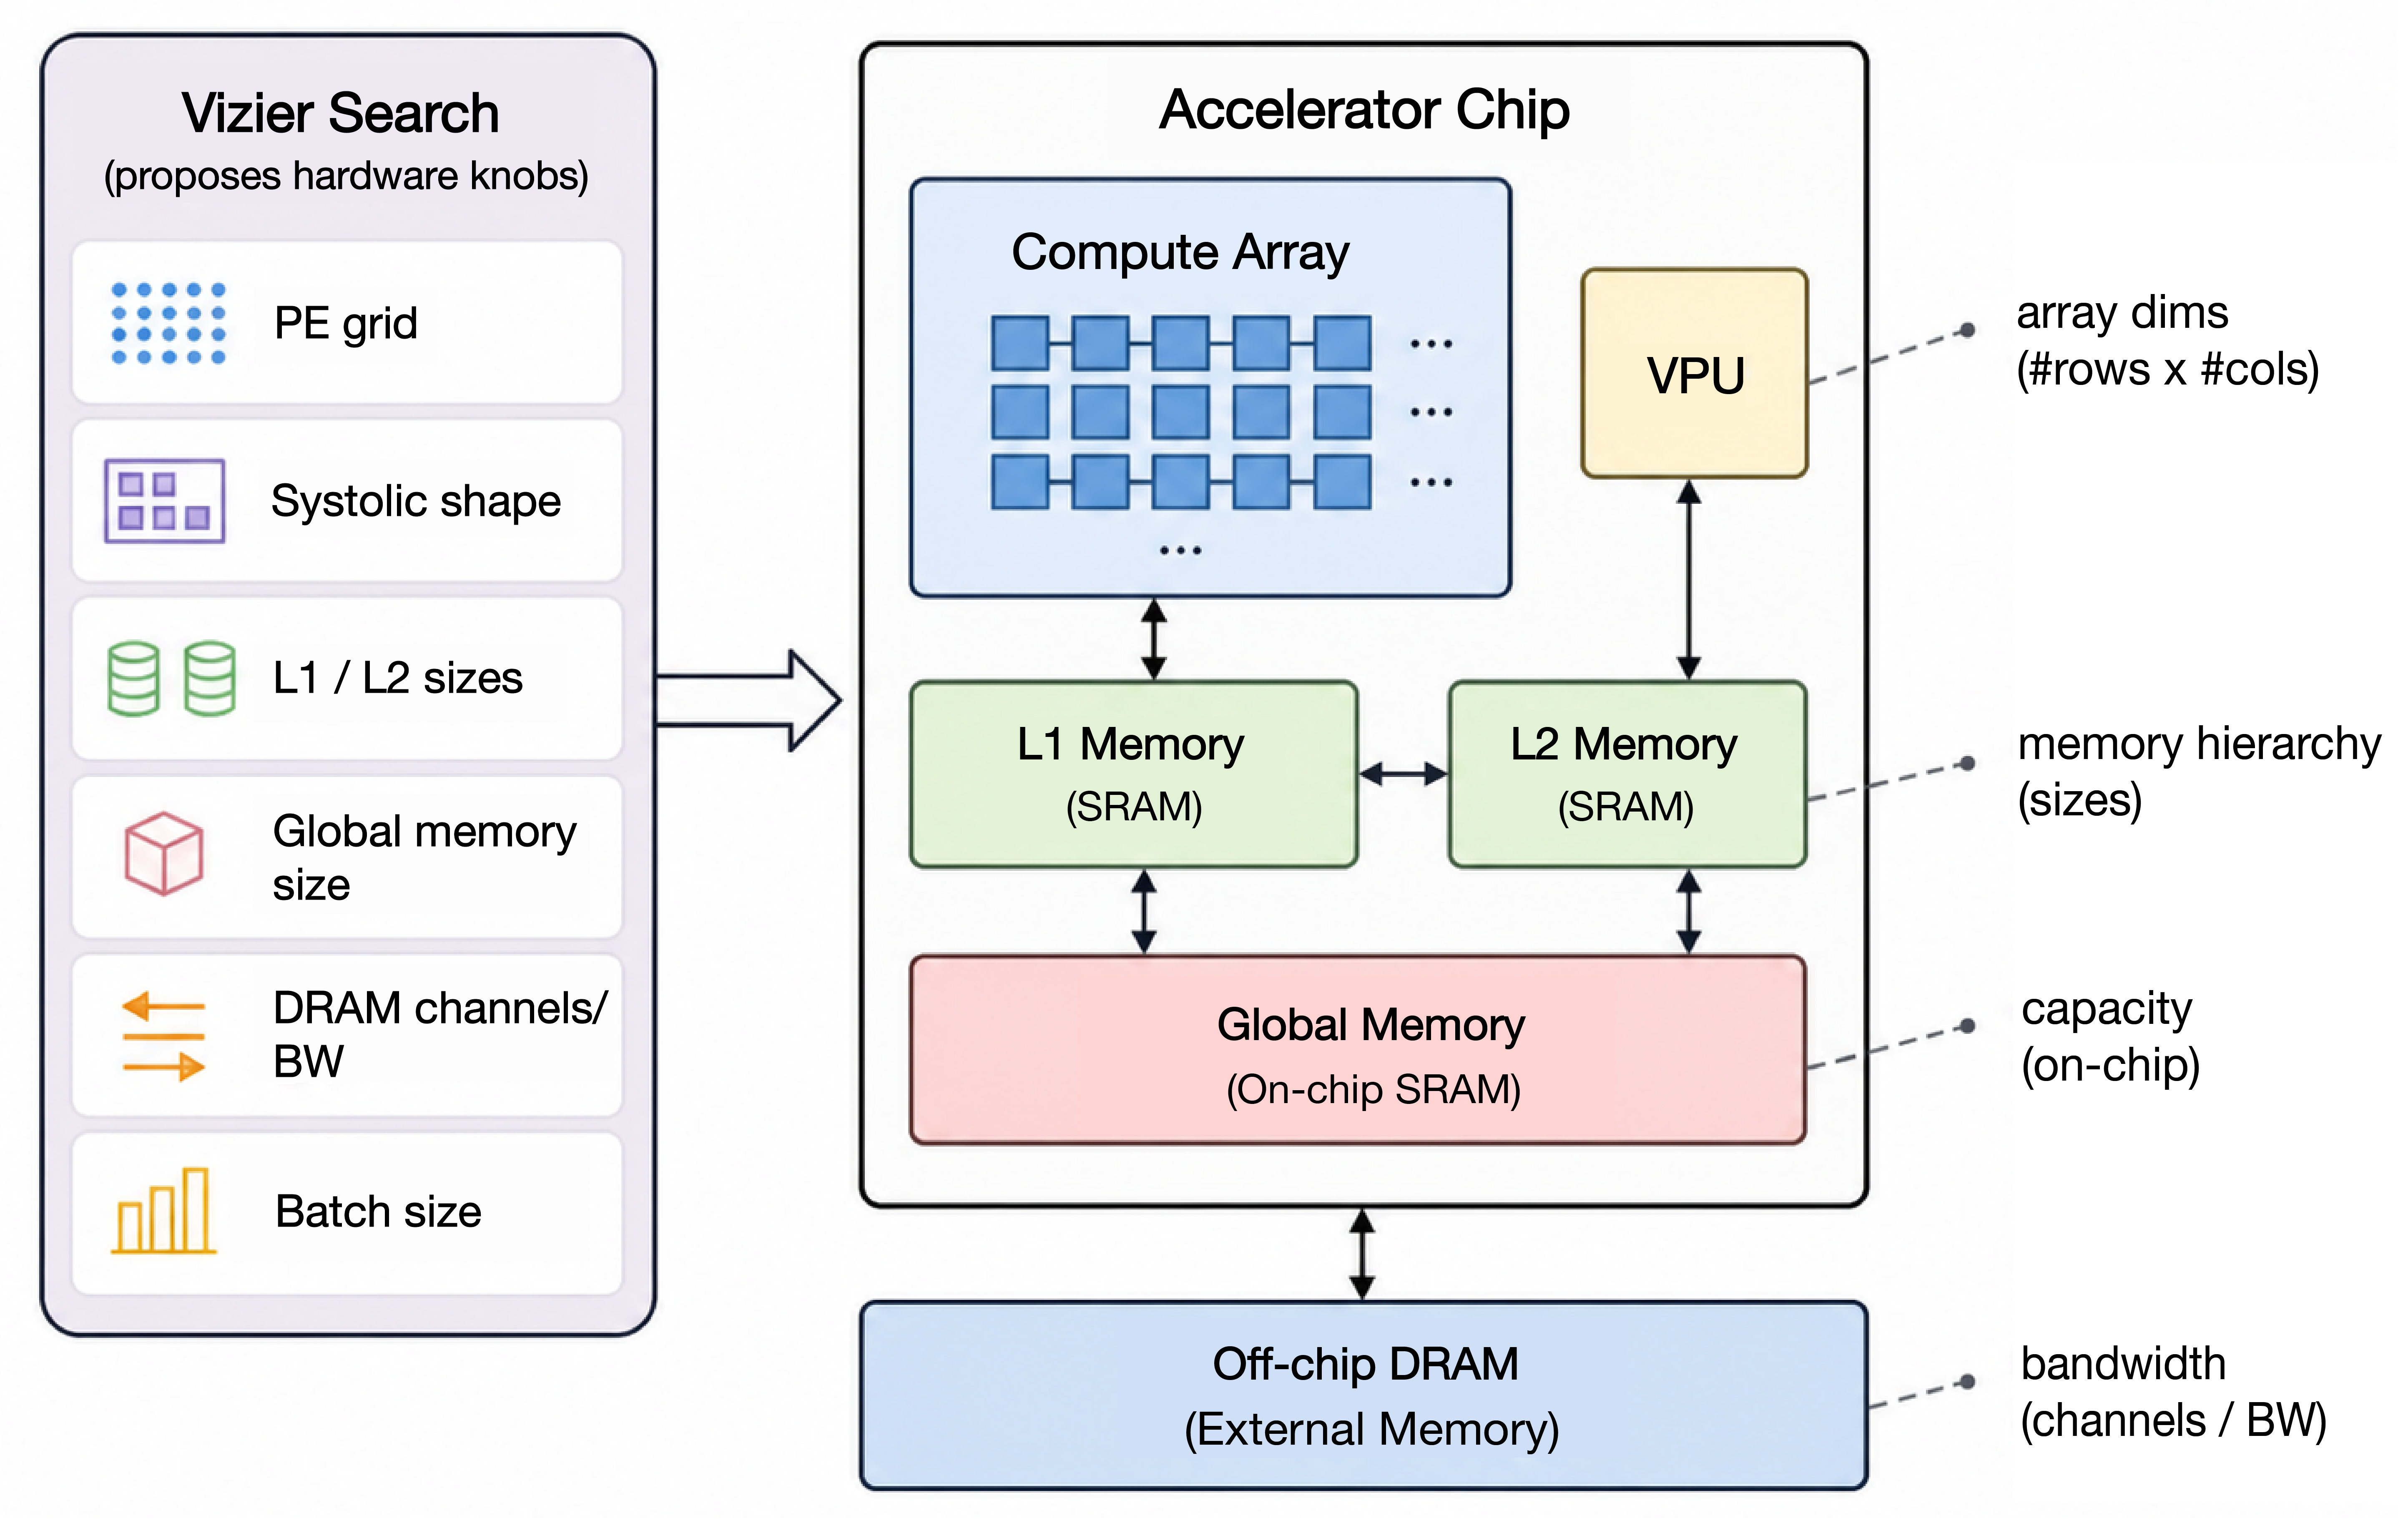
\includegraphics[width=0.7\linewidth]{figs/hardware_layout_v4.png}
%     \caption{The accelerator datapath configuration. Processing elements (PEs) are arranged in a grid connected by a mesh network. Each PE contains a systolic array for matrix operations, a vector processing unit (VPU) for non-MAC operations, and private or shared L1/L2 memory. A Global Memory serves as the on-chip scratchpad shared across all PEs.}
%     \label{fig:pipeline}
% \end{figure}
% \label{app:vizier}
% \begin{table}[h]
% \centering
% \caption{Vizier search parameter groups and ranges: initial small search vs.\ expanded V1-wide search.}
% \label{tab:vizier_search_space}
% \resizebox{\textwidth}{!}{%
% \begin{tabular}{llll}
% \toprule
% \textbf{Group} & \textbf{Parameter} & \textbf{Small (initial)} & \textbf{LLM-V1-wide} \\
% \midrule
% \multirow{16}{*}{\textbf{A — Hardware datapath (16 params)}}
%  & \texttt{PEs\_x\_dim}                & pow2 in $\mathbf{4 \ldots 32}$                          & pow2 in $\mathbf{1 \ldots 256}$                        \\
%  & \texttt{PEs\_y\_dim}                & pow2 in $\mathbf{4 \ldots 32}$                          & pow2 in $\mathbf{1 \ldots 256}$                        \\
%  & \texttt{Systolic\_array\_x}         & pow2 in $\mathbf{4 \ldots 32}$                          & pow2 in $\mathbf{4 \ldots 128}$                        \\
%  & \texttt{Systolic\_array\_y}         & pow2 in $\mathbf{4 \ldots 32}$                          & pow2 in $\mathbf{4 \ldots 128}$                        \\
%  & \texttt{Vector\_unit\_multiplier}   & pow2 $1 \ldots 16$                                      & pow2 $1 \ldots 16$                                     \\
%  & \texttt{L1\_buffer\_config}         & \{Private, Shared\}                                     & \{Private, Shared\}                                    \\
%  & \texttt{L1\_input\_buffer\_size}    & pow2 $\mathbf{1\,\text{KB} \ldots 4\,\text{MB}}$        & pow2 $\mathbf{1\,\text{KB} \ldots 1\,\text{MB}}$       \\
%  & \texttt{L1\_weight\_buffer\_size}   & pow2 $\mathbf{1\,\text{KB} \ldots 4\,\text{MB}}$        & pow2 $\mathbf{1\,\text{KB} \ldots 1\,\text{MB}}$       \\
%  & \texttt{L1\_output\_buffer\_size}   & pow2 $\mathbf{1\,\text{KB} \ldots 4\,\text{MB}}$        & pow2 $\mathbf{1\,\text{KB} \ldots 1\,\text{MB}}$       \\
%  & \texttt{L2\_buffer\_config}         & \{Disabled, Private, Shared\}                           & \{Disabled, Private, Shared\}                          \\
%  & \texttt{L2\_input\_buffer\_mult.}   & pow2 $1 \ldots 128$                                     & pow2 $1 \ldots 128$                                    \\
%  & \texttt{L2\_weight\_buffer\_mult.}  & pow2 $1 \ldots 128$                                     & pow2 $1 \ldots 128$                                    \\
%  & \texttt{L2\_output\_buffer\_mult.}  & pow2 $1 \ldots 128$                                     & pow2 $1 \ldots 128$                                    \\
%  & \texttt{L3\_global\_buffer} (CGM)   & $\{0\} \cup$ pow2 $\mathbf{1 \ldots 64\,\text{MB}}$     & $\{0\} \cup$ pow2 $\mathbf{1 \ldots 256\,\text{MB}}$   \\
%  & \texttt{GDDR6\_channels}            & pow2 $\mathbf{1 \ldots 16}$ ($\to$ 64–1024 GB/s)        & pow2 $\mathbf{1 \ldots 32}$ ($\to$ 64–2048 GB/s)       \\
%  & \texttt{Native\_batch\_size}        & pow2 $\mathbf{1 \ldots 1024}$                           & pow2 $\mathbf{1 \ldots 256}$                           \\
% \midrule
% \multirow{3}{*}{\textbf{B — Compiler passes (3 params)}}
%  & \texttt{two\_pass\_softmax}         & \{disabled, enabled\}                                   & \{disabled, enabled\}                                  \\
%  & \texttt{tensor\_padding}            & \{disabled, enabled\}                                   & \{disabled, enabled\}                                  \\
%  & \texttt{datatype}                   & \{bfloat16, int8\}                                      & \{bfloat16, int8\}                                     \\
% \midrule
% \multirow{2}{*}{\textbf{C — V0 rematerialisation (2 params)}}
%  & \texttt{remat\_enabled}             & \{disabled, enabled\}                                   & \{disabled, enabled\}                                  \\
%  & \texttt{remat\_cost\_scale}         & \{0.1, 0.25, 0.5, 1.0, 2.0, 4.0\}                      & \{0.1, 0.25, 0.5, 1.0, 2.0, 4.0\}                     \\
% \midrule
% \multirow{4}{*}{\textbf{D — V1 joint-tiling (4 params)}}
%  & \texttt{pareto\_config\_count\_C}   & \{10, 50, 100, 250, 500, 1000\}                         & \{10, 50, 100, 250, 500, 1000\}                        \\
%  & \texttt{loop\_ordering\_strategy}   & \{weight\_stationary, output\_stationary, both\}        & \{weight\_stationary, output\_stationary, both\}       \\
%  & \texttt{pareto\_pruning\_strategy}  & \{tmax\_workingset, tmax\_tmin, tmin\_workingset\}      & \{tmax\_workingset, tmax\_tmin, tmin\_workingset\}     \\
%  & \texttt{tile\_workingset\_modeling} & \{fixed, config\_dep\}                                  & \{fixed, config\_dep\}                                 \\
% \midrule
% \multirow{4}{*}{\textbf{Post-Vizier gates (filter, not search)}}
%  & \texttt{MIN\_TOTAL\_MACS}           & \multicolumn{2}{l}{$32{,}768$ ($4{\times}4{\times}4{\times}4{=}256$ lower physical, 32K gate)} \\
%  & \texttt{MAX\_TOTAL\_MACS} cap       & none — implicit $\leq 32{\times}32{\times}32{\times}32 \approx 1\,\text{M}$ & $1{,}048{,}576$ explicit cap \\
%  & Implied total\_MACs reach           & ${\approx}\,256 \ldots 1\,\text{M}$                     & $256 \ldots 1{,}048{,}576$ (post-cap)                  \\
%  & Implied DRAM BW reach               & $64 \ldots 1{,}024$ GB/s                                & $64 \ldots 2{,}048$ GB/s                               \\
% \bottomrule
% \end{tabular}%
% }
% \end{table}


\subsection{Why We Are Confident in the Software Side}
\label{app:sw_confidence}

The software claim is that the schedule the program commits to is the schedule
that runs, and that its optimality is bounded rather than asserted. Five
independent checks support it, ordered from strongest to weakest.

\paragraph{The committed schedule executes byte-exactly in RTL.}
The original DeepSeek-V3 validation schedule is compiled into a
$1{,}383$-instruction event tape
and executed on a cycle-accurate SystemVerilog engine under Verilator
(\cref{sec:rtl_validation}). The run completes with \textbf{zero} capacity
violations; the RTL peak on-chip occupancy equals the analytical prediction
\emph{exactly} at $7{,}602{,}176$~bytes; and the total cycle count lands within
$+0.000001\%$ of the rounded LP objective. This is the strongest form of the
claim available without silicon: the plan is not merely feasible on paper, it is
executable byte-for-byte on hardware that enforces the capacity constraint at
every step of that tape. This is not an RTL execution of the later
61,985,244-invocation native workload.

\paragraph{The checker is live, not vacuous.}
A validation suite is only meaningful if it can fail. We therefore replay a
deliberately over-committed tape, and the capacity checker flags exactly one
violation. A test that never fails proves nothing; this one fails when it should.

\paragraph{Optimality is bounded, not claimed.}
An admitted integral execution supplies a feasible endpoint under its modeled
contract. A lower bound applies only to the domain covered by its certificate;
working-support bounds cannot be promoted to the full library. The current
finite native family has a $21.6374\%$ continuous interval
(Appendix~\ref{app:native_provenance}). That interval is separate from the
recovered chip's predicted latency and is not a performance error bar.

\paragraph{Rounding is feasibility-preserving and independently validated.}
In the original campaign, relaxed selectors are rounded by enumeration over the physically integral
choices, and no pin that would violate a constraint is ever committed. Each
rounded design is re-solved and checked against the constraint set independently
of the solver that produced it, with residuals at the $10^{-13}$ level. We never
report a relaxed objective as an achievable result.

\paragraph{Search configurations remain explicit.}
The original campaign uses the configuration in
\cref{app:coeff_provenance}. The native extension separately records its
reference, recovered design, and matched controls in
Appendix~\ref{app:native_provenance}. Those controls share a chip and evaluator;
they are not globally optimized feature-off designs.

\paragraph{What this does not establish.}
RTL cycle counts are not used as an absolute oracle: the analytical per-layer
cache floors are conservative by $192\times$ to $2475\times$, so RTL evidence is
scoped to schedule realizability, memory legality, and utilization
\emph{mechanisms}. We make no claim that the simulated datapath is a
performance-optimal implementation.

\subsection{Why We Are Confident in the Hardware Side}
\label{app:hw_confidence}

The hardware evidence supports the declared cost-model mechanisms; it is not a
fabrication certificate for every modeled design. Design-space-exploration frameworks are conventionally validated
three ways, against measured taped-out chips, against post-synthesis extraction,
and against other frameworks~\citep{mei2021zigzag}. We have all three.

\paragraph{Against post-synthesis extraction: the area coefficient and its
functional form.}
We implement the scored datapath as synthesizable RTL and push it through
OpenROAD to placement at the ASAP7 $7$~nm predictive PDK
(\cref{sec:asap7}). Extracted cell area fits
$A = 82.08\,\mathrm{MACs} - 206.5\ \mu\mathrm{m}^2$ with $R^2 = 0.999999$, and
area per MAC varies by only $0.46\%$ across a $16\times$ range in MAC count. The
second number matters more than the first: the program assumes area is
\emph{linear with a size-independent slope}, and that is exactly what a placed
datapath exhibits. The coefficient we use is bracketed from below by extracted
cell area and from above by our own conservative floorplan.

\paragraph{Against shipped silicon: the energy coefficient.}
Our compute-energy coefficient corresponds to $0.40$~pJ per INT8 operation. Whole
chip figures for shipped accelerators are $0.35$ (H100), $0.64$ (A100) and
$1.27$~pJ/op (TPU-v4i), and an array-only coefficient must sit at or just below
whole-chip values. It does. We additionally measured the precision-energy ratio
directly rather than assuming it, and the measurement corrected our analytic
estimate in both directions (\cref{sec:energy_coeff}).

\paragraph{Against other frameworks: the mapping data.}
The original campaign's mapping data comes from Timeloop Pareto evaluations.
The native extension uses explicit analytical dispatch, primitive-service,
and memory-transfer contracts, as documented in
Appendix~\ref{app:native_provenance}.

\paragraph{Declared feasibility is checked.}
The original campaign enforces its six proxy gates. The native extension
checks its original LP rows, installed bank and staging resources, and
complete execution accounting. These are different evidence scopes; neither
replaces detailed physical implementation.

\paragraph{What this does not establish.}
We have not taped out, and we do not run clock-tree synthesis or routing, so we
make no claim about achievable clock frequency in silicon. Absolute power from
our own flow remains an upper bound rather than a prediction: an ungated tile
driven by uncorrelated data on a predictive PDK reports roughly three times our
coefficient, and we therefore anchor the coefficient to measured silicon rather
than to our own synthesis. The gating measurement in particular is not yet
trustworthy and no clock-gating decision is scored in the program as a result.
